\documentclass{article}
\usepackage{tikz}
\usetikzlibrary{patterns}
\usepackage{subcaption}
\usepackage[margin=1in]{geometry}

\begin{document}

\begin{figure}[ht]
    \centering
    \begin{subfigure}{0.45\textwidth}
        \centering
        \resizebox{\textwidth}{!}{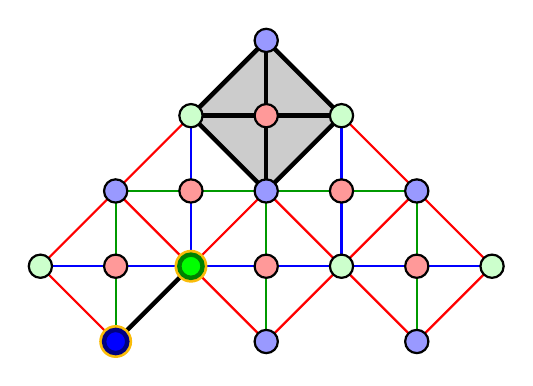
\begin{tikzpicture}[scale=0.7]
    \fill[gray!40] (-1.3657,4.0971) -- (0.0,2.7314) -- (0.0,4.0971) -- cycle;
    \fill[gray!40] (-1.3657,4.0971) -- (0.0,4.0971) -- (0.0,5.4628) -- cycle;
    \fill[gray!40] (0.0,2.7314) -- (0.0,4.0971) -- (1.3657,4.0971) -- cycle;
    \fill[gray!40] (0.0,4.0971) -- (0.0,5.4628) -- (1.3657,4.0971) -- cycle;
    \draw[blue, thick] (2.7314,1.3657) -- (4.0971,1.3657);
    \draw[blue, thick] (1.3657,2.7314) -- (1.3657,1.3657);
    \draw[blue, thick] (-1.3657,2.7314) -- (-1.3657,4.0971);
    \draw[blue, thick] (0.0,1.3657) -- (-1.3657,1.3657);
    \draw[black, ultra thick] (0.0,4.0971) -- (-1.3657,4.0971);
    \draw[blue, thick] (2.7314,1.3657) -- (1.3657,1.3657);
    \draw[blue, thick] (0.0,1.3657) -- (1.3657,1.3657);
    \draw[blue, thick] (-1.3657,2.7314) -- (-1.3657,1.3657);
    \draw[blue, thick] (-2.7314,1.3657) -- (-1.3657,1.3657);
    \draw[black, ultra thick] (0.0,4.0971) -- (1.3657,4.0971);
    \draw[blue, thick] (-2.7314,1.3657) -- (-4.0971,1.3657);
    \draw[blue, thick] (1.3657,2.7314) -- (1.3657,4.0971);
    \draw[black, ultra thick] (-1.3657,4.0971) -- (0.0,5.4628);
    \draw[black, ultra thick] (1.3657,4.0971) -- (0.0,2.7314);
    \draw[red, thick] (4.0971,1.3657) -- (2.7314,2.7314);
    \draw[black, ultra thick] (-1.3657,4.0971) -- (0.0,2.7314);
    \draw[red, thick] (1.3657,1.3657) -- (2.7314,0.0);
    \draw[black, ultra thick] (-1.3657,1.3657) -- (-2.7314,0.0);
    \draw[red, thick] (1.3657,4.0971) -- (2.7314,2.7314);
    \draw[red, thick] (-1.3657,1.3657) -- (0.0,0.0);
    \draw[red, thick] (1.3657,1.3657) -- (0.0,0.0);
    \draw[red, thick] (4.0971,1.3657) -- (2.7314,0.0);
    \draw[red, thick] (1.3657,1.3657) -- (0.0,2.7314);
    \draw[red, thick] (-4.0971,1.3657) -- (-2.7314,2.7314);
    \draw[red, thick] (-1.3657,1.3657) -- (0.0,2.7314);
    \draw[black, ultra thick] (1.3657,4.0971) -- (0.0,5.4628);
    \draw[red, thick] (-1.3657,1.3657) -- (-2.7314,2.7314);
    \draw[red, thick] (1.3657,1.3657) -- (2.7314,2.7314);
    \draw[red, thick] (-4.0971,1.3657) -- (-2.7314,0.0);
    \draw[red, thick] (-1.3657,4.0971) -- (-2.7314,2.7314);
    \draw[green!60!black, thick] (0.0,2.7314) -- (-1.3657,2.7314);
    \draw[green!60!black, thick] (-2.7314,2.7314) -- (-1.3657,2.7314);
    \draw[green!60!black, thick] (0.0,2.7314) -- (0.0,1.3657);
    \draw[black, ultra thick] (0.0,2.7314) -- (0.0,4.0971);
    \draw[green!60!black, thick] (-2.7314,2.7314) -- (-2.7314,1.3657);
    \draw[black, ultra thick] (0.0,5.4628) -- (0.0,4.0971);
    \draw[green!60!black, thick] (2.7314,2.7314) -- (1.3657,2.7314);
    \draw[green!60!black, thick] (-2.7314,0.0) -- (-2.7314,1.3657);
    \draw[green!60!black, thick] (0.0,2.7314) -- (1.3657,2.7314);
    \draw[green!60!black, thick] (0.0,0.0) -- (0.0,1.3657);
    \draw[green!60!black, thick] (2.7314,2.7314) -- (2.7314,1.3657);
    \draw[green!60!black, thick] (2.7314,0.0) -- (2.7314,1.3657);
    \filldraw[fill=yellow!50!orange, draw=none] (-2.7314, 0.0) circle (8.5pt);
    \filldraw[fill=blue, draw=blue!50!black, ultra thick] (-2.7314, 0.0) circle (6pt);
    \filldraw[fill=blue!40, draw=black, thick] (0.0, 0.0) circle (6pt);
    \filldraw[fill=blue!40, draw=black, thick] (2.7314, 0.0) circle (6pt);
    \filldraw[fill=blue!40, draw=black, thick] (-2.7314, 2.7314) circle (6pt);
    \filldraw[fill=blue!40, draw=black, thick] (0.0, 2.7314) circle (6pt);
    \filldraw[fill=blue!40, draw=black, thick] (2.7314, 2.7314) circle (6pt);
    \filldraw[fill=blue!40, draw=black, thick] (0.0, 5.4628) circle (6pt);
    \filldraw[fill=red!40, draw=black, thick] (-2.7314, 1.3657) circle (6pt);
    \filldraw[fill=red!40, draw=black, thick] (0.0, 1.3657) circle (6pt);
    \filldraw[fill=red!40, draw=black, thick] (2.7314, 1.3657) circle (6pt);
    \filldraw[fill=red!40, draw=black, thick] (-1.3657, 2.7314) circle (6pt);
    \filldraw[fill=red!40, draw=black, thick] (1.3657, 2.7314) circle (6pt);
    \filldraw[fill=red!40, draw=black, thick] (0.0, 4.0971) circle (6pt);
    \filldraw[fill=green!20, draw=black, thick] (-4.0971, 1.3657) circle (6pt);
    \filldraw[fill=yellow!50!orange, draw=none] (-1.3657, 1.3657) circle (8.5pt);
    \filldraw[fill=green, draw=green!50!black, ultra thick] (-1.3657, 1.3657) circle (6pt);
    \filldraw[fill=green!20, draw=black, thick] (1.3657, 1.3657) circle (6pt);
    \filldraw[fill=green!20, draw=black, thick] (4.0971, 1.3657) circle (6pt);
    \filldraw[fill=green!20, draw=black, thick] (-1.3657, 4.0971) circle (6pt);
    \filldraw[fill=green!20, draw=black, thick] (1.3657, 4.0971) circle (6pt);
\end{tikzpicture}
}
        \caption{Full Lattice (Errors in gray)}
    \end{subfigure}
    \hfill
    \begin{subfigure}{0.45\textwidth}
        \centering
        \resizebox{\textwidth}{!}{\input{boundary_fail_b.tex}}
        \caption{$\mathcal{L}_{RG}$ (MWPM matches to boundary)}
    \end{subfigure}
    
    \vspace{1cm}
    
    \begin{subfigure}{0.45\textwidth}
        \centering
        \resizebox{\textwidth}{!}{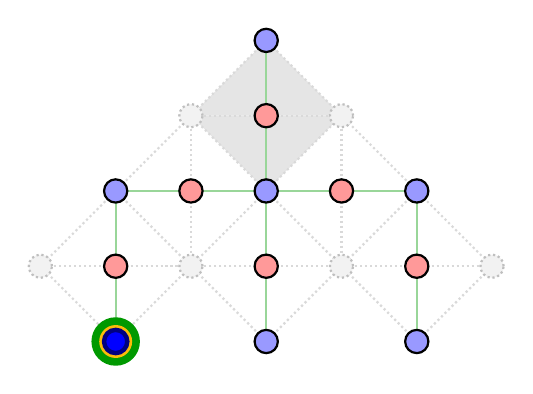
\begin{tikzpicture}[scale=0.7]
    \fill[gray!20] (-1.3657,4.0971) -- (0.0,2.7314) -- (0.0,4.0971) -- cycle;
    \fill[gray!20] (-1.3657,4.0971) -- (0.0,4.0971) -- (0.0,5.4628) -- cycle;
    \fill[gray!20] (0.0,2.7314) -- (0.0,4.0971) -- (1.3657,4.0971) -- cycle;
    \fill[gray!20] (0.0,4.0971) -- (0.0,5.4628) -- (1.3657,4.0971) -- cycle;
    \draw[gray!30, densely dotted, thick] (2.7314,1.3657) -- (4.0971,1.3657);
    \draw[gray!30, densely dotted, thick] (1.3657,2.7314) -- (1.3657,1.3657);
    \draw[gray!30, densely dotted, thick] (-1.3657,2.7314) -- (-1.3657,4.0971);
    \draw[gray!30, densely dotted, thick] (0.0,1.3657) -- (-1.3657,1.3657);
    \draw[gray!30, densely dotted, thick] (0.0,4.0971) -- (-1.3657,4.0971);
    \draw[gray!30, densely dotted, thick] (2.7314,1.3657) -- (1.3657,1.3657);
    \draw[gray!30, densely dotted, thick] (0.0,1.3657) -- (1.3657,1.3657);
    \draw[gray!30, densely dotted, thick] (-1.3657,2.7314) -- (-1.3657,1.3657);
    \draw[gray!30, densely dotted, thick] (-2.7314,1.3657) -- (-1.3657,1.3657);
    \draw[gray!30, densely dotted, thick] (0.0,4.0971) -- (1.3657,4.0971);
    \draw[gray!30, densely dotted, thick] (-2.7314,1.3657) -- (-4.0971,1.3657);
    \draw[gray!30, densely dotted, thick] (1.3657,2.7314) -- (1.3657,4.0971);
    \draw[gray!30, densely dotted, thick] (-1.3657,4.0971) -- (0.0,5.4628);
    \draw[gray!30, densely dotted, thick] (1.3657,4.0971) -- (0.0,2.7314);
    \draw[gray!30, densely dotted, thick] (4.0971,1.3657) -- (2.7314,2.7314);
    \draw[gray!30, densely dotted, thick] (-1.3657,4.0971) -- (0.0,2.7314);
    \draw[gray!30, densely dotted, thick] (1.3657,1.3657) -- (2.7314,0.0);
    \draw[gray!30, densely dotted, thick] (-1.3657,1.3657) -- (-2.7314,0.0);
    \draw[gray!30, densely dotted, thick] (1.3657,4.0971) -- (2.7314,2.7314);
    \draw[gray!30, densely dotted, thick] (-1.3657,1.3657) -- (0.0,0.0);
    \draw[gray!30, densely dotted, thick] (1.3657,1.3657) -- (0.0,0.0);
    \draw[gray!30, densely dotted, thick] (4.0971,1.3657) -- (2.7314,0.0);
    \draw[gray!30, densely dotted, thick] (1.3657,1.3657) -- (0.0,2.7314);
    \draw[gray!30, densely dotted, thick] (-4.0971,1.3657) -- (-2.7314,2.7314);
    \draw[gray!30, densely dotted, thick] (-1.3657,1.3657) -- (0.0,2.7314);
    \draw[gray!30, densely dotted, thick] (1.3657,4.0971) -- (0.0,5.4628);
    \draw[gray!30, densely dotted, thick] (-1.3657,1.3657) -- (-2.7314,2.7314);
    \draw[gray!30, densely dotted, thick] (1.3657,1.3657) -- (2.7314,2.7314);
    \draw[gray!30, densely dotted, thick] (-4.0971,1.3657) -- (-2.7314,0.0);
    \draw[gray!30, densely dotted, thick] (-1.3657,4.0971) -- (-2.7314,2.7314);
    \draw[green!60!black!40, thick] (0.0,2.7314) -- (-1.3657,2.7314);
    \draw[green!60!black!40, thick] (-2.7314,2.7314) -- (-1.3657,2.7314);
    \draw[green!60!black!40, thick] (0.0,2.7314) -- (0.0,1.3657);
    \draw[green!60!black!40, thick] (0.0,2.7314) -- (0.0,4.0971);
    \draw[green!60!black!40, thick] (-2.7314,2.7314) -- (-2.7314,1.3657);
    \draw[green!60!black!40, thick] (0.0,5.4628) -- (0.0,4.0971);
    \draw[green!60!black!40, thick] (2.7314,2.7314) -- (1.3657,2.7314);
    \draw[green!60!black!40, thick] (-2.7314,0.0) -- (-2.7314,1.3657);
    \draw[green!60!black!40, thick] (0.0,2.7314) -- (1.3657,2.7314);
    \draw[green!60!black!40, thick] (0.0,0.0) -- (0.0,1.3657);
    \draw[green!60!black!40, thick] (2.7314,2.7314) -- (2.7314,1.3657);
    \draw[green!60!black!40, thick] (2.7314,0.0) -- (2.7314,1.3657);
    \filldraw[fill=none, draw=green!60!black, line width=3.5pt] (-2.7314,0.0) circle (10pt);
    \filldraw[fill=yellow!50!orange, draw=none] (-2.7314, 0.0) circle (8.5pt);
    \filldraw[fill=blue, draw=blue!50!black, ultra thick] (-2.7314, 0.0) circle (6pt);
    \filldraw[fill=blue!40, draw=black, thick] (0.0, 0.0) circle (6pt);
    \filldraw[fill=blue!40, draw=black, thick] (2.7314, 0.0) circle (6pt);
    \filldraw[fill=blue!40, draw=black, thick] (-2.7314, 2.7314) circle (6pt);
    \filldraw[fill=blue!40, draw=black, thick] (0.0, 2.7314) circle (6pt);
    \filldraw[fill=blue!40, draw=black, thick] (2.7314, 2.7314) circle (6pt);
    \filldraw[fill=blue!40, draw=black, thick] (0.0, 5.4628) circle (6pt);
    \filldraw[fill=red!40, draw=black, thick] (-2.7314, 1.3657) circle (6pt);
    \filldraw[fill=red!40, draw=black, thick] (0.0, 1.3657) circle (6pt);
    \filldraw[fill=red!40, draw=black, thick] (2.7314, 1.3657) circle (6pt);
    \filldraw[fill=red!40, draw=black, thick] (-1.3657, 2.7314) circle (6pt);
    \filldraw[fill=red!40, draw=black, thick] (1.3657, 2.7314) circle (6pt);
    \filldraw[fill=red!40, draw=black, thick] (0.0, 4.0971) circle (6pt);
    \filldraw[fill=gray!10, draw=gray!50, densely dotted, thick] (-4.0971, 1.3657) circle (6pt);
    \filldraw[fill=gray!10, draw=gray!50, densely dotted, thick] (-1.3657, 1.3657) circle (6pt);
    \filldraw[fill=gray!10, draw=gray!50, densely dotted, thick] (1.3657, 1.3657) circle (6pt);
    \filldraw[fill=gray!10, draw=gray!50, densely dotted, thick] (4.0971, 1.3657) circle (6pt);
    \filldraw[fill=gray!10, draw=gray!50, densely dotted, thick] (-1.3657, 4.0971) circle (6pt);
    \filldraw[fill=gray!10, draw=gray!50, densely dotted, thick] (1.3657, 4.0971) circle (6pt);
\end{tikzpicture}
}
        \caption{$\mathcal{L}_{RB}$ (MWPM matches to boundary)}
    \end{subfigure}
    \hfill
    \begin{subfigure}{0.45\textwidth}
        \centering
        \resizebox{\textwidth}{!}{\input{boundary_fail_d.tex}}
        \caption{$\mathcal{L}_{GB}$ (MWPM matches correctly)}
    \end{subfigure}
    \vspace{1cm}
    
    \begin{subfigure}{0.45\textwidth}
        \centering
        \resizebox{\textwidth}{!}{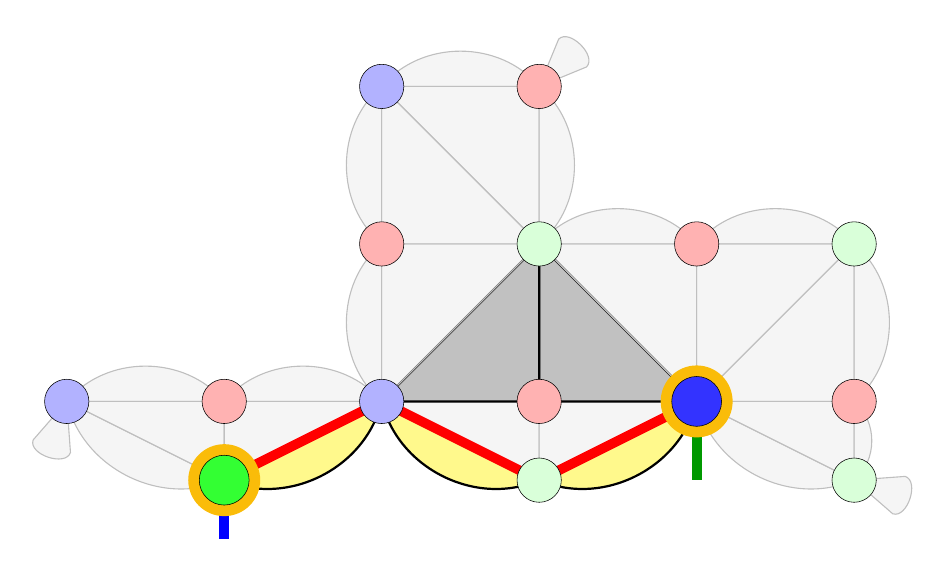
\begin{tikzpicture}[scale=0.5]
    \filldraw[fill=gray!15, draw=gray!50, , fill opacity=0.5] (1,3) -- (1.095,1.703) to[bend left=90] (0.146,2.020) -- cycle;
    \filldraw[fill=gray!15, draw=gray!50, , fill opacity=0.5] (1,3) to[bend right=50] (5,1) -- cycle;
    \filldraw[fill=yellow!50, draw=black, thick, fill opacity=0.9] (9,3) to[bend left=50] (5,1) -- cycle;
    \filldraw[fill=yellow!50, draw=black, thick, fill opacity=0.9] (9,3) to[bend right=50] (13,1) -- cycle;
    \filldraw[fill=yellow!50, draw=black, thick, fill opacity=0.9] (17,3) to[bend left=50] (13,1) -- cycle;
    \filldraw[fill=gray!15, draw=gray!50, , fill opacity=0.5] (17,3) to[bend right=50] (21,1) -- cycle;
    \filldraw[fill=gray!15, draw=gray!50, , fill opacity=0.5] (21,1) -- (22.297,1.095) to[bend left=90] (21.980,0.146) -- cycle;
    \filldraw[fill=gray!15, draw=gray!50, , fill opacity=0.5] (5,1) -- (5,3) -- (1,3) -- cycle;
    \filldraw[fill=gray!15, draw=gray!50, , fill opacity=0.5] (5,1) -- (9,3) -- (5,3) -- cycle;
    \filldraw[fill=gray!15, draw=gray!50, , fill opacity=0.5] (13,1) -- (13,3) -- (9,3) -- cycle;
    \filldraw[fill=gray!15, draw=gray!50, , fill opacity=0.5] (13,1) -- (17,3) -- (13,3) -- cycle;
    \filldraw[fill=gray!15, draw=gray!50, , fill opacity=0.5] (21,1) -- (21,3) -- (17,3) -- cycle;
    \filldraw[fill=gray!15, draw=gray!50, , fill opacity=0.5] (21,3) to[bend left=50] (21,1) -- cycle;
    \filldraw[fill=gray!15, draw=gray!50, , fill opacity=0.5] (5,3) to[bend right=50] (1,3) -- cycle;
    \filldraw[fill=gray!15, draw=gray!50, , fill opacity=0.5] (5,3) to[bend left=50] (9,3) -- cycle;
    \filldraw[fill=gray!60, draw=black, thick, fill opacity=0.8] (9,3) -- (13,3) -- (13,7) -- cycle;
    \filldraw[fill=gray!60, draw=black, thick, fill opacity=0.8] (13,3) -- (17,3) -- (13,7) -- cycle;
    \filldraw[fill=gray!15, draw=gray!50, , fill opacity=0.5] (17,3) -- (21,3) -- (21,7) -- cycle;
    \filldraw[fill=gray!15, draw=gray!50, , fill opacity=0.5] (21,3) to[bend right=50] (21,7) -- cycle;
    \filldraw[fill=gray!15, draw=gray!50, , fill opacity=0.5] (9,7) to[bend right=50] (9,3) -- cycle;
    \filldraw[fill=gray!15, draw=gray!50, , fill opacity=0.5] (9,3) -- (13,7) -- (9,7) -- cycle;
    \filldraw[fill=gray!15, draw=gray!50, , fill opacity=0.5] (17,3) -- (17,7) -- (13,7) -- cycle;
    \filldraw[fill=gray!15, draw=gray!50, , fill opacity=0.5] (17,3) -- (21,7) -- (17,7) -- cycle;
    \filldraw[fill=gray!15, draw=gray!50, , fill opacity=0.5] (9,7) to[bend left=50] (9,11) -- cycle;
    \filldraw[fill=gray!15, draw=gray!50, , fill opacity=0.5] (9,7) -- (13,7) -- (9,11) -- cycle;
    \filldraw[fill=gray!15, draw=gray!50, , fill opacity=0.5] (17,7) to[bend right=50] (13,7) -- cycle;
    \filldraw[fill=gray!15, draw=gray!50, , fill opacity=0.5] (17,7) to[bend left=50] (21,7) -- cycle;
    \filldraw[fill=gray!15, draw=gray!50, , fill opacity=0.5] (13,7) -- (13,11) -- (9,11) -- cycle;
    \filldraw[fill=gray!15, draw=gray!50, , fill opacity=0.5] (13,11) to[bend left=50] (13,7) -- cycle;
    \filldraw[fill=gray!15, draw=gray!50, , fill opacity=0.5] (13,11) to[bend right=50] (9,11) -- cycle;
    \filldraw[fill=gray!15, draw=gray!50, , fill opacity=0.5] (13,11) -- (13.495,12.202) to[bend left=90] (14.202,11.495) -- cycle;
    \draw[blue, line width=3.5pt] (5,1) -- (5, -0.5);
    \draw[green!60!black, line width=3.5pt] (17,3) -- (17,1);
    \draw[red, line width=3.5pt] (5,1) -- (9,3) -- (13,1) -- (17,3);
    \filldraw[fill=red!30, draw=black, very thin] (5, 3) circle (16pt);
    \filldraw[fill=red!30, draw=black, very thin] (13, 3) circle (16pt);
    \filldraw[fill=red!30, draw=black, very thin] (21, 3) circle (16pt);
    \filldraw[fill=red!30, draw=black, very thin] (9, 7) circle (16pt);
    \filldraw[fill=red!30, draw=black, very thin] (17, 7) circle (16pt);
    \filldraw[fill=red!30, draw=black, very thin] (13, 11) circle (16pt);
    \filldraw[fill=blue!30, draw=black, very thin] (9, 3) circle (16pt);
    \filldraw[fill=yellow!50!orange, draw=none] (17, 3) circle (26pt);
    \filldraw[fill=blue!80, draw=black, very thin] (17, 3) circle (18pt);
    \filldraw[fill=green!15, draw=black, very thin] (13, 7) circle (16pt);
    \filldraw[fill=blue!30, draw=black, very thin] (1, 3) circle (16pt);
    \filldraw[fill=blue!30, draw=black, very thin] (9, 11) circle (16pt);
    \filldraw[fill=green!15, draw=black, very thin] (21, 7) circle (16pt);
    \filldraw[fill=yellow!50!orange, draw=none] (5, 1) circle (26pt);
    \filldraw[fill=green!80, draw=black, very thin] (5, 1) circle (18pt);
    \filldraw[fill=green!15, draw=black, very thin] (13, 1) circle (16pt);
    \filldraw[fill=green!15, draw=black, very thin] (21, 1) circle (16pt);
\end{tikzpicture}
}
        \caption{Projection Decoder (Logical Failure)}
    \end{subfigure}
    \hfill
    \begin{subfigure}{0.45\textwidth}
        \centering
        \resizebox{\textwidth}{!}{\input{boundary_fail_f.tex}}
        \caption{Restriction Lift $\mathcal{L}_{RG} \cup \mathcal{L}_{RB}$}
    \end{subfigure}
    \caption{Visual example of boundary failure in the Projection Decoder. An error chain parallel to the boundary produces a syndrome that MWPM matches to the boundary in two projections, but pairs together in the third, resulting in a logical failure upon recombination.}
\end{figure}

\end{document}
